\documentclass[10pt]{extarticle}

% Lingua e matematica
\usepackage[english]{babel}
\usepackage{amsmath,amssymb,amsthm}

% Grafica e tabelle
\usepackage{graphicx}
\usepackage{subcaption}
\usepackage{float}
\usepackage{booktabs}
\usepackage{multirow}
\usepackage{siunitx}

% Codice (opzionale)
\usepackage{listings}
\usepackage{xcolor}
\definecolor{codegreen}{rgb}{0,0.6,0}
\definecolor{codegray}{rgb}{0.5,0.5,0.5}
\definecolor{codepurple}{rgb}{0.58,0,0.82}
\definecolor{backcolour}{rgb}{0.98,0.98,0.98}
\lstdefinestyle{mystyle}{
  backgroundcolor=\color{backcolour},
  commentstyle=\color{codegreen},
  keywordstyle=\color{magenta},
  numberstyle=\tiny\color{codegray},
  stringstyle=\color{codepurple},
  basicstyle=\ttfamily\footnotesize,
  breaklines=true, keepspaces=true, numbers=none, tabsize=2
}
\lstset{style=mystyle}

% Margini
\usepackage[margin=0.6in]{geometry}
\usepackage{ragged2e}
\usepackage{enumitem}
%\usepackage[utf8]{inputenc} % per caratteri UTF-8 nei .tex e nel .bib
\usepackage[backend=biber,style=ieee,sorting=none,maxbibnames=99]{biblatex}
\ExecuteBibliographyOptions{doi=true,url=true,isbn=false}
\addbibresource{references.bib}
\usepackage{csquotes}       % consigliato da biblatex (evita warning e parse strani)



% Bibliografia (biblatex + biber)
\usepackage[backend=biber,style=ieee]{biblatex}
\addbibresource{references.bib}

% TOC: includi anche \paragraph e numerali
\setcounter{secnumdepth}{2}
\setcounter{tocdepth}{2}

% Hyperref (sempre *dopo* gli altri pacchetti)
\usepackage[colorlinks=true,linkcolor=blue,citecolor=teal,urlcolor=magenta]{hyperref}


\begin{document}

% Custom header without a separate titlepage
\noindent
\begin{minipage}{0.3\textwidth}
    
\includegraphics[width=1.3\linewidth]{Figures/polito_logo_2021_blu.jpg}
\end{minipage}
\hfill
\begin{minipage}{0.68\textwidth}
    \raggedleft
    {\LARGE \textbf{Politecnico di Torino}}\\[0.2cm]
    {\large Master's Degree in Mathematical Engineering}\\[0.7cm]
    {\large \textbf{Material for Thesis}}\\[0.2cm]
    {\large 1-- Medical and Biological Information}\\[0.7cm]
    \begin{tabular}{rl}
        Elisabetta Roviera & \texttt{s328422} \\
    \end{tabular}
\end{minipage}

\vspace{1cm}
\hrule
\vspace{0.5cm}

\tableofcontents

\vspace{0.5cm}
\hrule
\vspace{1cm}


% Main content begins here, on the same page
\justifying

\paragraph{Note} 
The papers summarized in this report currently represent the main references consulted for the medical and biological background of the thesis, with a focus on cancer biology and epigenetic mechanisms. Additional papers may be reviewed in the future if further clinical or molecular details become necessary. For a complete understanding of the concepts and results discussed, consult the original publications, all of which are cited in the bibliography of this document.


\section{Understanding Cancer}  
\paragraph{Keywords} Cancer biology, tumorigenesis, oncogenes, tumor suppressor genes, epidemiology, multistep process, cell proliferation, genetic mutations, clonal evolution, molecular pathways \cite{NIH2007}

\paragraph{Understanding Cancer} Cancer is a disease of unregulated cell growth and division, ultimately leading to the ability of cells to invade tissues and metastasize. Unlike normal cells, which follow strict regulatory signals to balance proliferation and differentiation, cancer cells escape these controls and gain a selective advantage within their environment. This aberrant behavior reflects cumulative genetic and epigenetic alterations that disrupt normal cellular programs, making cancer both a genetic disease and a disorder of tissue organization.

\paragraph{Clues from Epidemiology}
Epidemiological studies provide critical insights into cancer development, showing that incidence increases markedly with age and varies across populations depending on environmental exposures. Carcinogens such as tobacco, ultraviolet radiation, and dietary factors elevate risk by introducing mutations or promoting conditions favorable to malignant transformation. Familial cancer syndromes further demonstrate the hereditary component of tumorigenesis, as inherited mutations can predispose individuals to malignancies by effectively bypassing early steps in the carcinogenic process.

\paragraph{Clues from Cell Biology}
From a cell biology perspective, malignant transformation is linked to fundamental changes in cellular behavior. Cancer cells display reduced dependence on growth factors, insensitivity to inhibitory signals, and the ability to proliferate indefinitely through mechanisms such as telomerase activation. They also evade apoptosis, tolerate genomic instability, and acquire the capacity to invade surrounding tissue. These phenotypic alterations highlight the breakdown of cellular safeguards that normally prevent uncontrolled proliferation.

\paragraph{Cancer as a Multistep Process}
Cancer progression follows a multistep evolutionary model, in which successive genetic alterations accumulate over time. Each step provides additional growth advantages, leading to the selection of increasingly aggressive clones. This process explains the long latency of most cancers and the exponential rise in incidence with age. Figure \ref{fig:stages_tumor} illustrates this concept, depicting the sequential acquisition of mutations and their correspondence with distinct stages of tumor progression, from normal tissue to invasive carcinoma.

\begin{figure}[h]
    \centering
    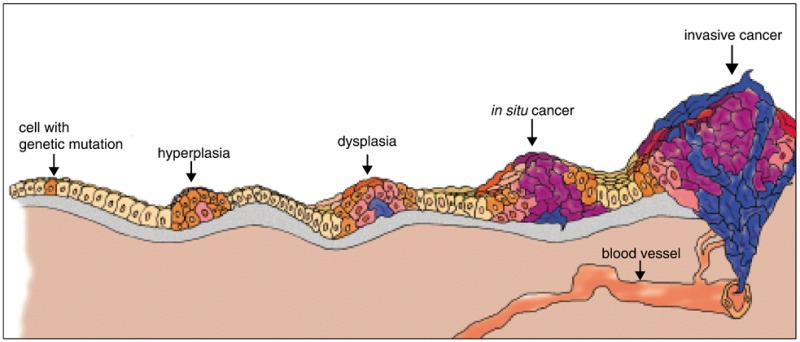
\includegraphics[width=0.7\textwidth]{Figures/Different_phases_of_tumor.jpg} % o .png, .pdf, .eps...
    \caption{The stages of tumor development.}
    \label{fig:stages_tumor}
\end{figure}


\paragraph{The Role of Tumor Suppressor Genes}
Among the critical genetic regulators are tumor suppressor genes, which function as the cellular “brakes” to counterbalance proliferative signals. The loss or inactivation of these genes—exemplified by p53 or RB—removes essential checkpoints in the cell cycle, permits survival of damaged cells, and enhances genomic instability. Their role complements that of oncogenes, underscoring that cancer arises not from a single lesion but from the interplay between multiple disrupted pathways. Together, these insights provide a coherent framework for understanding cancer as a progressive, multistep disease shaped by both genetic predisposition and environmental exposure.

\section{Introduction to Cancer Biology}

\paragraph{Keywords} Tumor biology, cancer hallmarks, cell proliferation, apoptosis, angiogenesis, metastasis, immune evasion, telomerase \cite{azizi2022introduction}

\paragraph{Foundations of Tumor Biology}
Cancer is a multifactorial and heterogeneous disease involving complex interactions at cellular, tissue, and organismic levels. Malignant tumors evolve through Darwinian selection, where advantageous genetic and epigenetic alterations enable clonal expansion of malignant cells. The tumor microenvironment—including stromal and immune cells—contributes to cancer initiation, progression, and systemic dissemination. Hanahan and Weinberg’s model of the \textit{hallmarks of cancer} remains central to the understanding of tumor biology, outlining the key capabilities acquired during tumorigenesis.

\paragraph{Constitutive Proliferation}
Normal cell proliferation is tightly regulated by growth-promoting and inhibitory signals to maintain homeostasis. In cancer, mutations deregulate these mechanisms, allowing autonomous and continuous proliferation. Examples include activating mutations in EGFR, B-Raf (V600E), and Ras, as well as PTEN promoter methylation, which disrupts negative feedback and enhances PI3K/AKT/mTOR signaling. These molecular defects collectively ensure uncontrolled cell division, impaired apoptosis, and tumor growth.

\paragraph{Resistance to Growth Inhibition and Cell Death}
Cancer cells evade growth suppressors such as RB1 and TP53, bypassing cell-cycle checkpoints and apoptosis. Mutations in these tumor suppressors lead to genomic instability and uncontrolled replication. Tumors also suppress programmed cell death by overexpressing anti-apoptotic proteins (e.g., Bcl-2) and inhibiting pro-apoptotic factors. Additionally, alterations in autophagy and necroptosis pathways enable cancer cells to survive under stress, resist therapy, and maintain malignancy.

\paragraph{Escaping Replicative Mortality}
Senescence and telomere shortening normally limit cell lifespan, but cancer cells bypass these barriers via reactivation of telomerase (TERT). Telomerase elongates telomeres, preventing DNA damage-induced senescence or apoptosis, while also supporting WNT, MYC, and NF-kB signaling pathways. These noncanonical functions promote stemness, epithelial–mesenchymal transition (EMT), and metastatic potential, establishing telomerase as a hallmark of cellular immortality in cancer.

\paragraph{Inducing Angiogenesis}
Tumor growth requires sustained vascularization to supply oxygen and nutrients. The “angiogenic switch” favors proangiogenic signaling through VEGF, PDGF, FGF, and MMPs, which remodel the extracellular matrix (ECM) and promote endothelial cell proliferation. Hypoxia-induced stabilization of HIF-1$\alpha$ further enhances VEGF expression, sustaining neovascularization. This process, though essential for tumor expansion, also facilitates metastasis by providing vascular access for invasive cells.

\paragraph{Invasion, Metastasis, and Immune Modulation}
Metastasis arises when tumor cells undergo EMT, lose adhesion, and invade surrounding tissues. Matrix-degrading enzymes (MMPs, uPA) and exosome-mediated communication promote intravasation and dissemination as circulating tumor cells (CTCs). Once in circulation, CTC clusters exhibit enhanced survival and metastatic potential. In parallel, tumors modulate the immune microenvironment by recruiting regulatory T cells, myeloid-derived suppressor cells, and M2 macrophages that suppress cytotoxic responses through TGF-$\beta$, VEGF, and IL-10. This immunosuppressive state facilitates immune escape, angiogenesis, and metastatic colonization.

\section{The Hallmarks of Cancer}

\paragraph{Keywords} Hallmarks of cancer, tumor biology, cell signaling, oncogenes, tumor suppressor genes, apoptosis, angiogenesis, metastasis  \cite{hanahan2000hallmarks}

\paragraph{Introduction}
The authors proposed a unifying conceptual framework for understanding tumorigenesis. They identified six essential physiological traits—termed \textit{acquired capabilities}—that characterize the transformation of normal cells into malignant ones. These hallmarks, summarized in Figure \ref{fig:capab_tumor}, include: (1) self-sufficiency in growth signals, (2) insensitivity to antigrowth signals, (3) evasion of apoptosis, (4) limitless replicative potential, (5) sustained angiogenesis, and (6) tissue invasion and metastasis. Together, these alterations enable uncontrolled cell proliferation and are common to virtually all human cancers.

\begin{figure}[h]
    \centering
    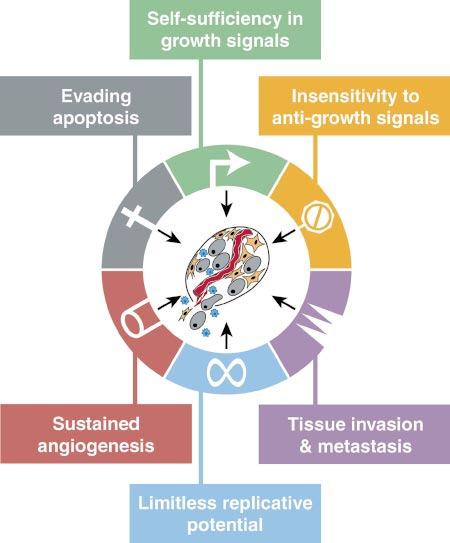
\includegraphics[width=0.3\textwidth]{Figures/Acquired Capabilities of Cancer.jpg} % o .png, .pdf, .eps...
    \caption{We suggest that most if not all cancers have acquired the same set of functional capabilities during their development, albeit through various mechanistic strategies.}
    \label{fig:capab_tumor}
\end{figure}

\paragraph{Self-Sufficiency in Growth Signals}
Normal cells depend on external mitogenic signals to proliferate, but cancer cells bypass this requirement. They often produce their own growth factors (\textit{autocrine stimulation}), overexpress or mutate growth factor receptors such as EGFR or HER2, and activate downstream signaling cascades like the Ras–Raf–MAPK pathway. This independence from external stimuli grants continuous proliferative signaling. Figure~3 further expands this view by emphasizing that tumors co-opt surrounding stromal cells to release paracrine growth factors, illustrating that tumor growth involves both autonomous and microenvironment-driven signaling.

\paragraph{Insensitivity to Antigrowth Signals}
Normal tissues maintain homeostasis through antiproliferative cues mediated by the \textit{Rb pathway} and factors such as TGF-$\beta$. Cancer cells acquire resistance by mutating components like \textit{RB1}, \textit{CDK4}, or \textit{Smad4}, or by downregulating TGF-$\beta$ receptors. These disruptions abolish cell-cycle checkpoints and allow continuous entry into the S-phase. Additionally, altered adhesion molecules and integrins suppress inhibitory signaling, reinforcing unrestrained growth.

\paragraph{Evasion of Apoptosis}
Apoptosis normally removes damaged or abnormal cells. Tumor cells disable this defense by mutating \textit{TP53}—a key sensor of DNA damage—or by upregulating anti-apoptotic proteins such as Bcl-2 and Bcl-XL. Pro-survival pathways like PI3K/AKT are frequently activated, while death receptors (e.g., FAS) are downregulated or inhibited by decoy receptors. This resistance to programmed cell death permits the accumulation of genetic lesions and enhances tumor resilience.

\paragraph{Limitless Replicative Potential}
Normal somatic cells are restricted by telomere shortening, which induces senescence and crisis. Cancer cells bypass this limit through reactivation of telomerase (TERT) or alternative lengthening of telomeres (ALT) mechanisms, preserving chromosome stability and enabling immortal proliferation. Telomere maintenance thus represents a universal requirement for tumor progression and clonal expansion.

\paragraph{Sustained Angiogenesis}
Tumors require oxygen and nutrients beyond a diffusion limit of 100 µm, necessitating new vasculature formation. The “angiogenic switch” (Figure \ref{fig:capab_tumor}) involves overexpression of proangiogenic factors such as VEGF and FGF, and suppression of inhibitors like thrombospondin-1. Loss of p53 further favors angiogenesis by reducing inhibitory signaling. This neovascularization is critical for tumor growth and provides routes for metastasis.

\paragraph{Tissue Invasion and Metastasis}
The final hallmark enables tumor cells to breach local barriers and colonize distant tissues. Key molecular events include loss of E-cadherin-mediated adhesion, altered integrin expression, and activation of matrix metalloproteinases (MMPs). These changes degrade the extracellular matrix and facilitate migration. As shown in Figure \ref{fig:complex_tumor}, cancer is increasingly recognized as an ecosystem in which malignant cells recruit stromal, endothelial, and immune cells that cooperate in invasion and metastasis.

\begin{figure}[h]
    \centering
    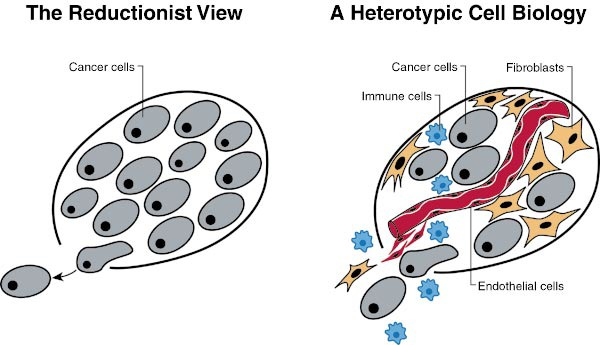
\includegraphics[width=0.4\textwidth]{Figures/Tumors as Complex Tissues.jpg} % o .png, .pdf, .eps...
    \caption{The field of cancer research has largely been
guided by a reductionist focus on cancer cells
and the genes within them (left panel)—a focus
that has produced an extraordinary body
of knowledge. Looking forward in time, we
believe that important new inroads will come
from regarding tumors as complex tissues in
which mutant cancer cells have conscripted
and subverted normal cell types to serve as
active collaborators in their neoplastic agenda
(right panel). The interactions between the
genetically altered malignant cells and these
supporting coconspirators will prove critical
to understanding cancer pathogenesis and to
the development of novel, effective therapies.}
    \label{fig:complex_tumor}
\end{figure}

\paragraph{Conclusion}
The six acquired capabilities represent a conceptual framework linking the genetic complexity of cancer to a finite set of functional traits. Hanahan and Weinberg’s model (Figure \ref{fig:capab_tumor}) has transformed oncology by providing a logical map of tumor evolution—from normalcy to malignancy—and by emphasizing the interplay between cell-autonomous mutations and the tumor microenvironment illustrated in Figure \ref{fig:complex_tumor}.

\section{DNA Methylation in Cancer: Too Much, but Also Too Little}

\paragraph{Keywords} DNA methylation, hypomethylation, hypermethylation, CpG islands, satellite DNA, LINE-1, epigenetic instability, oncogenesis  \cite{ehrlich2002dna}

\paragraph{Introduction}
The authors revisit the dual epigenetic imbalance in cancer, emphasizing that both global DNA hypomethylation and localized hypermethylation coexist as hallmarks of malignancy. While hypermethylation of CpG islands in tumor suppressor gene promoters is well recognized for its silencing effect, global hypomethylation—often more extensive—has received less attention despite its widespread presence across various cancer types. Hypomethylation affects repetitive elements, heterochromatic regions, and even single-copy genes, contributing independently to oncogenic transformation and genomic instability.

\paragraph{Global DNA Hypomethylation}
Early studies revealed substantial reductions in 5-methylcytosine (m5C) content in malignant tissues compared with normal counterparts. These decreases are especially pronounced in metastatic and aggressive tumors. Hypomethylation is detected in multiple cancers—colon, ovarian, prostate, liver, and Wilms tumors—indicating that genome-wide undermethylation is a general feature of cancer. Repetitive DNA sequences such as LINE-1, Alu, HERV-K retroelements, and satellite DNA (Sat2, Sat3, $\alpha$-satellite) are among the most affected. Their demethylation may activate transposons or disrupt chromatin condensation, fostering chromosomal rearrangements and karyotypic instability that drive tumor progression.

\paragraph{Localized Hypermethylation of CpG Islands}
In contrast, cancer-associated hypermethylation typically targets CpG islands within promoter regions of tumor suppressor genes. This modification induces transcriptional silencing of critical regulators such as \textit{RB1}, \textit{p16}, \textit{VHL}, and \textit{BRCA1}. High-throughput analyses estimate that hundreds to thousands of CpG islands are hypermethylated in specific tumor types, particularly colon and breast cancers. These patterns are tissue-specific and occur independently of hypomethylation, suggesting distinct underlying mechanisms for each epigenetic alteration.

\paragraph{Sequences Affected by Hypomethylation}
Ehrlich categorizes hypomethylation into several genomic contexts. Highly repeated sequences (e.g., LINE-1, Alu) lose methylation, potentially leading to retrotransposition or transcriptional interference. Moderately repeated elements, including endogenous retroviruses (HERV-K) and pericentromeric repeats, become transcriptionally active in cancers such as bladder, testicular, and hepatocellular carcinoma. Satellite DNA hypomethylation, particularly of centromeric and juxtacentromeric regions, is strongly correlated with chromosomal instability and structural aberrations like 1q gain and 16q loss. Furthermore, single-copy genes—including \textit{c-MYC}, \textit{HOX11}, \textit{pS2}, and \textit{MN/CA9}—exhibit promoter hypomethylation that coincides with aberrant overexpression, reinforcing the link between demethylation and oncogene activation.

\paragraph{Functional Consequences and Mechanisms}
Cancer-associated hypomethylation contributes to tumorigenesis through both \textit{cis} and \textit{trans} effects. \textit{Cis}-acting hypomethylation directly upregulates oncogenes or growth-promoting genes, while \textit{trans} effects arise from altered heterochromatin-euchromatin interactions that globally dysregulate gene expression. Loss of methylation in satellite DNA and retrotransposons destabilizes chromatin structure, promoting recombination, translocation, and amplification events. The resulting genomic instability accelerates tumor evolution and heterogeneity.

\paragraph{Hypo- and Hypermethylation in Cancer Progression}
Ehrlich concludes that hypomethylation and hypermethylation represent two complementary but mechanistically independent pathways in cancer epigenetics. Hypermethylation silences tumor suppressors, removing inhibitory controls, while hypomethylation activates proto-oncogenes and destabilizes the genome. Together, they create a permissive epigenetic environment for malignant transformation. Although demethylating drugs may transiently reactivate silenced genes, non-specific DNA demethylation could paradoxically enhance tumor progression by promoting genomic instability. Thus, understanding both hyper- and hypomethylation is essential for the safe and effective design of epigenetic cancer therapies.

\section{DNA Methylation Patterns and Epigenetic Memory}

\paragraph{Keywords}
Epigenetic memory, DNA methylation, CpG islands, DNMT1, DNMT3A, DNMT3B, transcriptional silencing, genomic imprinting, chromatin regulation \cite{bird2002dna}

\paragraph{Introduction}
The authors explores the biological logic of DNA methylation as a mechanism of epigenetic memory that preserves transcriptional states during mammalian development. While transcription factors initiate gene-specific activation or repression, stable maintenance of cell identity requires heritable mechanisms independent of DNA sequence. DNA methylation fulfills this role by copying epigenetic information through mitosis, ensuring that patterns of gene expression—once established—are remembered across cell generations. A definition of epigenetics
is: “The study of mitotically and/or meiotically
heritable changes in gene function that cannot be explained
by changes in DNA sequence” \cite{russo1996epigenetic}. 

\paragraph{Variability and Distribution of DNA Methylation}
Animal species display broad variability in genomic methylation levels, ranging from almost complete absence in \textit{C. elegans} to pervasive methylation in vertebrates. Mammalian genomes show a global methylation pattern with distinct unmethylated CpG islands located at promoter regions of approximately 60\% of genes. These islands remain unmethylated even in transcriptionally silent contexts, while bulk non-island DNA tends to be methylated. Developmental demethylation and remethylation cycles, particularly in early embryos and germ cells, establish the long-term methylation landscape that dictates tissue-specific expression and imprinting.

\paragraph{Maintenance Methylation}
Maintenance methylation preserves the methylation state during DNA replication. The enzyme DNMT1 preferentially methylates hemimethylated CpG sites on the daughter strand, propagating parental methylation patterns. However, experimental observations reveal that the process is imperfect—errors occur in 4–5\% of CpGs per division. Despite this, domain-level stability persists, implying additional factors beyond DNMT1 ensure faithful inheritance. Even in DNMT1-deficient cells, some CpG island methylation remains stable, indicating auxiliary maintenance mechanisms or chromatin-based cues reinforce methylation memory.

\paragraph{Consequences of Methylation Gain: Stable Gene Silencing}
De novo methylation confers heritable transcriptional silencing, locking previously repressed genes into an inactive state. In mammals, DNA methylation participates in processes such as X-chromosome inactivation, genomic imprinting, and repression of germline-specific genes (e.g., \textit{MAGE} family). Methylation ensures the irreversibility of gene silencing, as demethylating agents like 5-azacytidine can reactivate inactivated genes. Mechanistically, repression occurs either by blocking transcription factor binding or by recruiting methyl-CpG-binding proteins (MeCP2, MBD1–4, Kaiso) that attract histone deacetylase complexes, reinforcing closed chromatin architecture.



\paragraph{Mechanisms of Methylation-Mediated Repression}
Two complementary mechanisms explain transcriptional repression by methylation: (1) steric interference with transcription factor binding at methylated CpG sites, exemplified by CTCF regulation of the \textit{H19/Igf2} locus; and (2) recruitment of methyl-CpG-binding proteins that remodel chromatin into an inactive state. These pathways convert reversible silencing into a stable, heritable modification that contributes to long-term gene repression.

\paragraph{Excluding DNA Methylation and the Origin of CpG Islands}
Not all genomic regions are methylated. CpG islands remain protected through active transcription or chromatin accessibility, preventing DNMT access. Bird proposes that promoter activity during embryogenesis imprints unmethylated CpG islands that persist throughout life as potential sites for transcriptional reactivation. In contrast, inactive regions become methylated, creating enduring transcriptional barriers. Thus, CpG islands act as molecular records of early developmental transcriptional activity and represent an epigenetic memory of promoter competence.

\paragraph{Consequences of Methylation Loss}
Hypomethylation during development can lead to gene activation or genomic instability. Experimental deletion of \textit{Dnmt1} in mouse cells causes widespread gene activation, particularly of tissue-specific genes, indicating that methylation normally suppresses inappropriate expression. However, demethylation may also destabilize the genome, promoting chromosomal rearrangements or reactivation of transposable elements such as LINEs and IAPs. Therefore, methylation loss exerts dual effects—beneficial for reprogramming but potentially oncogenic when uncontrolled.

\paragraph{Epigenetic Memory and the Parallel with Polycomb/Trithorax}
Bird concludes that DNA methylation functions analogously to Polycomb/Trithorax (Pc-G/trx) complexes, both serving as cellular memory systems that preserve transcriptional states without initiating them. Methylation marks regions already silenced, ensuring the permanence of repression, while active promoters retain unmethylated CpG islands. Together, these systems form complementary mechanisms for epigenetic inheritance.

\paragraph{Conclusion: From Development to Disease}
DNA methylation encodes developmental memory by stabilizing gene expression patterns. In cancer, the same principles are pathologically co-opted: hypermethylation locks tumor suppressor genes in silence, whereas global hypomethylation erases epigenetic constraints, activating transposons and inducing genomic instability. The balance between these opposing forces—too much and too little methylation—thus determines both normal cellular identity and malignant transformation.

\section{The CpG Landscape of Protein Coding DNA in Vertebrates}

\paragraph{Keywords}
CpG dinucleotide, DNA methylation, protein coding DNA, genetic code, codon usage, GC content, vertebrate genomes \cite{wilcox2025cpg}

\paragraph{Introduction}
The authors investigate the evolutionary implications of CpG dinucleotides in vertebrate protein-coding DNA. The study combines theoretical analysis of the standard genetic code with comparative genomics across six species—human, mouse, chicken, great tit, frog, and stickleback—to explore how CpG sites are distributed and maintained in coding sequences. DNA methylation at CpG sites promotes cytosine deamination, causing a characteristic depletion of CpG motifs across vertebrate genomes. However, CpGs persist in specific regulatory or coding regions, suggesting functional importance despite mutational pressure. Notably, CpG content is consistently higher in protein-coding genes than in noncoding DNA, implying selective retention of these dinucleotides in functionally constrained loci.

\paragraph{The Genetic Code and CpG Dinucleotides}
Within the standard genetic code, CpG dinucleotides may occur either within individual codons or across adjacent codons (Figure \ref{fig:CpG}). CpG methylation alters mutation dynamics, biasing substitutions toward TpG or CpA and influencing amino acid coding potential. Theoretical modeling shows that CpG-containing codons can encode five amino acids—arginine (R), serine (S), proline (P), threonine (T), and alanine (A)—with varying degrees of redundancy. The genetic code therefore permits CpG dinucleotides but does not require them, making CpG the only facultative dinucleotide in the code.

\begin{figure}[h]
    \centering
    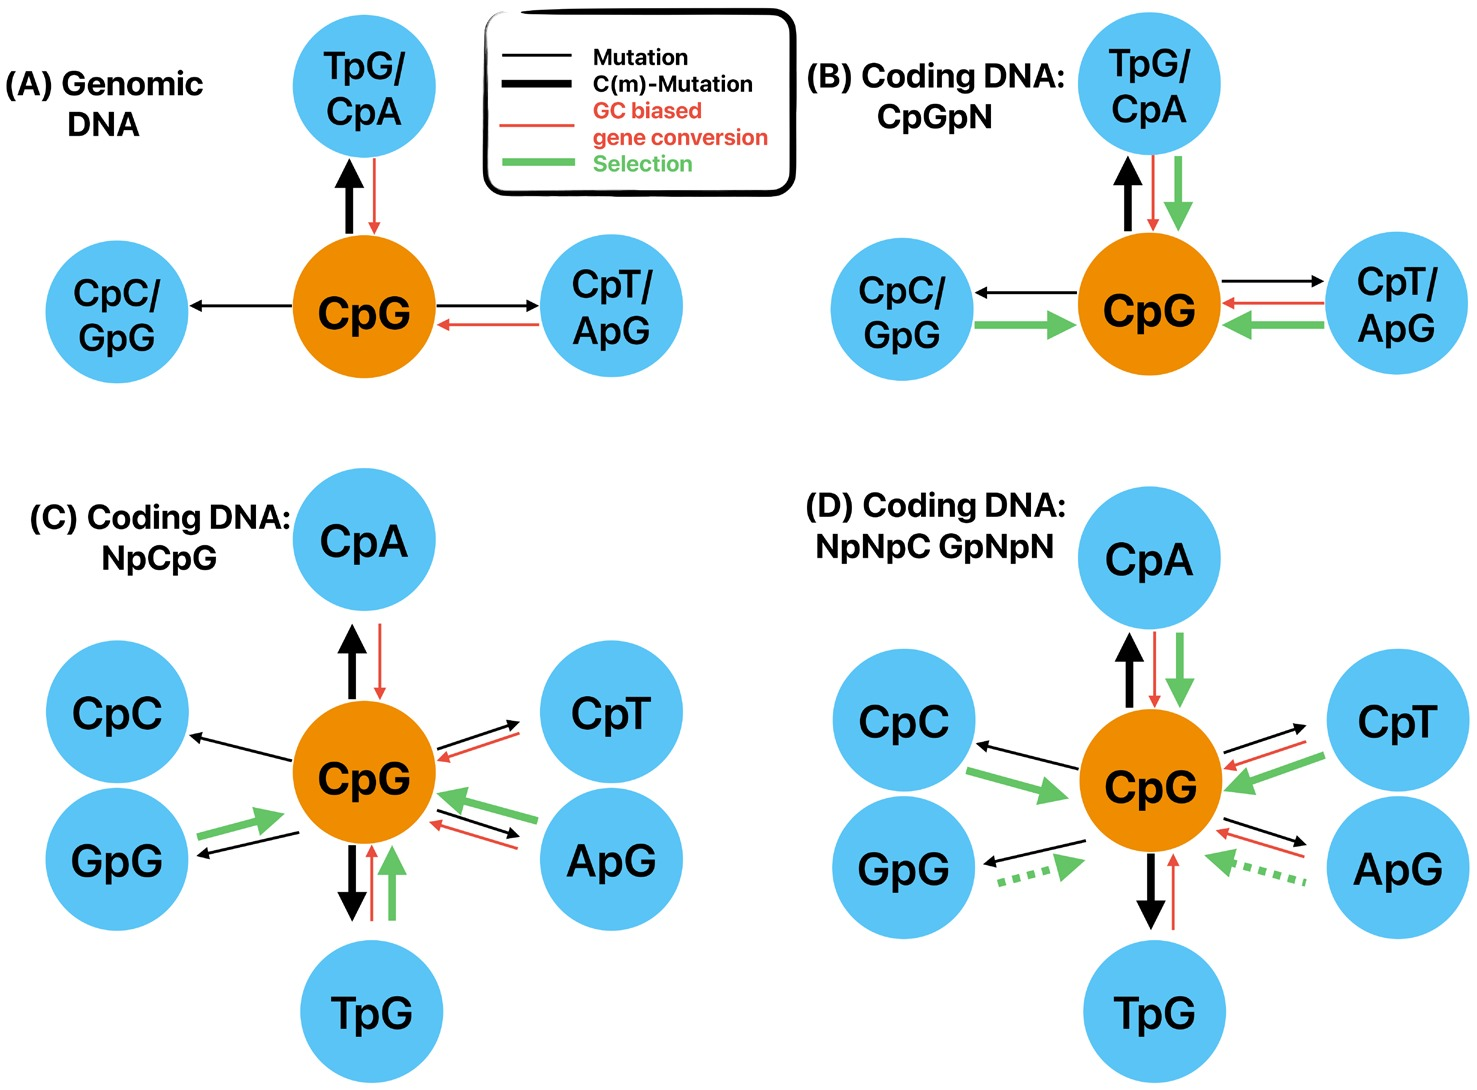
\includegraphics[width=0.4\textwidth]{Figures/Evolutionary forces acting on CpG dinucleotides.jpg} % o .png, .pdf, .eps...
    \caption{Evolutionary forces acting on CpG dinucleotides. (A) CpG sites in a genomic context (B–D) CpG sites in coding DNA context. C(m)-Mutation
denote a methylation dependent mutation rate}
    \label{fig:CpG}
\end{figure}

\paragraph{CpG Dinucleotides Within Codons}
CpG sites occurring at the first and second codon positions (CpGpN) invariably encode arginine. Methylation-driven mutations at these positions (e.g., CpG→TpG or CpG→CpA) generate nonsynonymous substitutions, often introducing deleterious amino acid changes or premature stop codons. Such mutations are subject to purifying selection, whereas GC-biased gene conversion tends to restore C–G pairs, partially counteracting CpG loss. Conversely, CpG sites at the second–third codon positions (NCpG) are found in codons encoding serine, proline, threonine, and alanine, where mutations at the third base are frequently synonymous and thus selectively tolerated.

\paragraph{CpG Dinucleotides Across Codons}
CpG motifs can also span adjacent codons (i.e., between a C-terminating codon and a G-starting codon). In these cases, CpG→TpG mutations are typically synonymous and produce non-CpG alternatives for the same dipeptide, reducing functional impact. Nevertheless, mutations at cross-codon CpGs can occasionally generate nonsynonymous substitutions, especially when the downstream codon begins with G. The ability to avoid CpG sites while maintaining amino acid identity reveals strong evolutionary flexibility in the coding potential of vertebrate genomes.

\paragraph{Any CpG Dinucleotide Can Be Replaced in the Standard Genetic Code}
Analyses of the standard genetic code show that any protein can, in principle, be encoded entirely without CpG dinucleotides. Among the 61 sense codons, eight contain CpG within codons, while fifteen can form CpGs across codon boundaries. Substituting these with CpG-free alternatives reduces the codon set to 38 unique CpG-free codons, still sufficient to encode all 20 amino acids. The code thus offers a mechanism to minimize CpG usage where selective or mutational pressures favor avoidance. However, GC-biased selection or structural constraints may preserve CpG-rich codons in certain proteins.

\paragraph{CpG Content}
To quantify CpG enrichment, the authors defined CpG content as the ratio of CpG to total C/G-containing palindromic dinucleotides (CpG + GpC). Comparative analysis across vertebrates revealed that CpG content is significantly higher in protein-coding DNA than in whole-genome averages ($p\leq 10^4$). Furthermore, CpG frequency correlates positively with overall GC content, though genes with exceptionally high CpG levels often occur in regions of intermediate GC composition—suggesting selective maintenance rather than compositional bias. These results imply that CpG motifs play a role in gene regulation, translational optimization, and possibly chromatin accessibility near transcription start sites.

\paragraph{Meaning of the Term “CpG”}
The abbreviation “CpG” stands for “cytosine–phosphate–guanine.” The “p” represents the \textbf{phosphodiester bond} linking the $5'$-carbon of cytosine to the $3'$-carbon of guanine in the DNA backbone. Unlike “CG” base pairs across strands, “CpG” specifically denotes a $5'$–$3'$ linear dinucleotide on the same strand, the canonical substrate for DNA methylation. CpG methylation occurs predominantly at the cytosine base, forming 5-methylcytosine (5mC), a key epigenetic mark affecting gene regulation and mutational dynamics.




\section{Breast Cancer}

\paragraph{Keywords} Breast cancer, epidemiology, pathophysiology, risk factors, histopathology, BRCA, molecular subtypes \cite{menon2025breast}

\paragraph{Continuing Education Activity}
Breast cancer is the most common malignancy among women and the second leading cause of cancer-related mortality worldwide. It accounts for more than 10\% of new cancer diagnoses annually. The disease often develops silently and is typically detected through screening programs, particularly in Western countries. Early detection and multimodal treatment—combining surgery, radiotherapy, chemotherapy, hormonal, and immunotherapy—have significantly improved overall survival and patient outcomes. This educational review aims to strengthen healthcare professionals’ competence in recognizing risk factors, differentiating breast cancer types, and implementing effective management strategies through interprofessional collaboration.

\paragraph{Introduction}
The breast is an exocrine gland composed of lobes and lobules that produce and transport milk through lactiferous ducts. Breast cancer primarily originates from the ductal epithelium (ductal carcinoma) or, less frequently, from lobular tissue (lobular carcinoma). In Western countries, most breast cancers are detected through screening rather than symptoms, while in developing regions they often present as palpable masses or nipple discharge. Diagnosis relies on clinical examination, imaging, and histopathological confirmation, and therapy is tailored according to tumor type, stage, hormonal status, and genetic markers.

\paragraph{Etiology}
Breast cancer arises from a multifactorial interplay of genetic, hormonal, and environmental factors. Established risk factors include advancing age, female sex, personal or family history of breast cancer, and histologic abnormalities such as lobular carcinoma in situ and atypical hyperplasia. Germline mutations in \textit{BRCA1} and \textit{BRCA2} account for 5–10\% of all cases, but up to 25\% in women under 30. Reproductive factors that increase lifetime estrogen exposure—early menarche, nulliparity, late menopause, or first childbirth after age 30—elevate risk, as do exogenous hormones, obesity, alcohol, and radiation exposure.

\paragraph{Epidemiology}
Globally, breast cancer accounts for approximately 11.7\% of all new cancer diagnoses (2020 data). In the United States, one in eight women and one in a thousand men will develop the disease. Incidence increases with age, peaking in women aged 75–79 years, with a median diagnosis age of 61. Mortality has declined markedly in developed countries thanks to early detection and improved therapies—by about 43\% between 1980 and 2020—yet disparities persist: African American women experience higher mortality despite a slightly lower incidence than non-Hispanic whites. In contrast, rates are still increasing in parts of Africa and Asia due to limited access to screening and treatment.

\paragraph{Pathophysiology}
The majority (90–95\%) of breast cancers are sporadic, while 5–10\% are hereditary. Tumor development reflects interactions between genetic susceptibility, hormonal influence, and environmental exposures. Molecular profiling identifies four major subtypes: Luminal A (ER/PR+, HER2–), Luminal B (ER/PR+, HER2+), HER2-enriched (HER2+, ER/PR–), and Basal-like or triple-negative (ER–/PR–/HER2–). Luminal tumors are generally less aggressive and respond to hormonal therapy, whereas HER2-enriched and basal-like subtypes are associated with poorer prognosis and higher metastatic potential, though targeted anti-HER2 therapy (e.g., trastuzumab) has markedly improved outcomes.

\paragraph{Histopathology}
Invasive breast cancer is characterized by neoplastic cell invasion beyond the basement membrane and encompasses diverse histologic subtypes. The most prevalent form, invasive ductal carcinoma, represents 50–75\% of cases and arises from the terminal duct-lobular unit. Invasive lobular carcinoma (10–15\%) exhibits single-file cell infiltration and often evades detection until advanced. Less common subtypes include mucinous (2–5\%), tubular (1–2\%), and medullary carcinomas, the latter being more frequent in younger or BRCA-mutant patients. Pathologic evaluation includes hormone receptor (ER, PR) and HER2 testing, Ki-67 proliferation index, grade, and morphology, all of which guide therapeutic decisions and prognosis.

\begin{figure}[h]
    \centering
    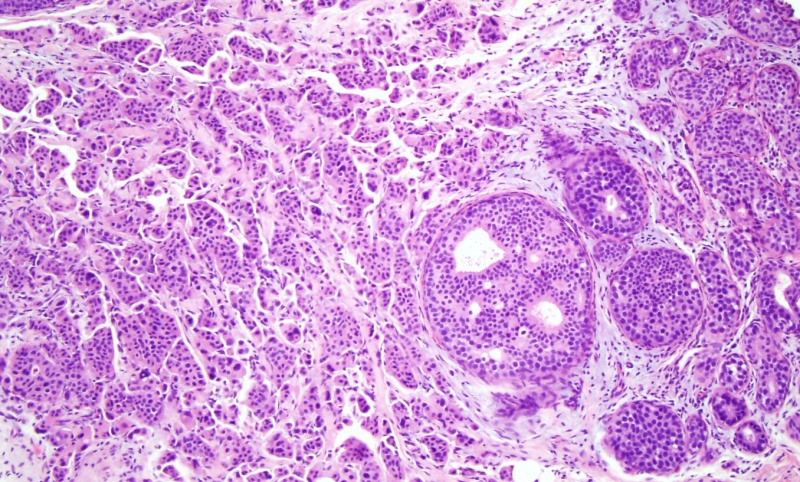
\includegraphics[width=0.5\textwidth]{Figures/Invasive Ductal Carcinoma..jpg} % o .png, .pdf, .eps...
    \caption{Invasive Ductal Carcinoma. Histological slide of high-grade ductal carcinoma in situ with invasive ductal carcinoma (×10). The left side of the image shows a sheet of cells with pleomorphic nuclei, arranged in tubules, infiltrating into the breast stroma, consistent with invasive ductal carcinoma originating from the adjacent high-grade ductal carcinoma in situ on the right side of the image. Contributed by M Khan, DO}
    \label{fig:invasive_tumore}
\end{figure}





\section{BRCA Gene Changes: Cancer Risk and Genetic Testing}

\paragraph{Keywords} BRCA1, BRCA2, breast cancer, ovarian cancer, hereditary cancer, genetic testing, DNA repair  \cite{nci_brca_2024}

\paragraph{BRCA Genes and DNA Repair Mechanisms}
The BRCA1 (BReast CAncer gene 1) and BRCA2 (BReast CAncer gene 2) genes encode proteins that play a crucial role in repairing damaged DNA and preserving genomic integrity. Each individual inherits two copies of these genes, one from each parent. A harmful inherited mutation, also called a pathogenic variant, compromises the cell’s DNA repair capacity and increases the likelihood of developing multiple cancers, particularly breast and ovarian cancer. Although one normal allele typically provides protection, a somatic alteration in the remaining copy can trigger complete loss of repair function and subsequent tumor formation.

\paragraph{Cancer Risks Associated with BRCA Mutations}
Women carrying pathogenic variants in BRCA1 or BRCA2 exhibit lifetime breast cancer risks exceeding 60\%, compared with about 13\% in the general population. Likewise, 39–58\% of BRCA1 carriers and 13–29\% of BRCA2 carriers develop ovarian cancer, compared with 1.1\% among women without such mutations. Among breast cancer survivors, mutation carriers also show a substantially higher probability of developing contralateral breast cancer within 20 years of their first diagnosis.

\paragraph{BRCA Mutations in Men and Other Associated Cancers}
Although less common, men with BRCA mutations are also predisposed to cancer. Approximately 0.2–1.2\% of BRCA1 and 1.8–7.1\% of BRCA2 male carriers develop breast cancer by age 70, compared with 0.1\% in the general male population. In addition, BRCA mutations are linked to increased susceptibility to pancreatic, prostate, melanoma, and rare endometrial cancers, underscoring their broad oncogenic potential.

\paragraph{Population Differences and Founder Mutations}
The frequency of BRCA mutations varies across populations. In the general population, approximately 0.2–0.3\% of individuals carry pathogenic variants, but the prevalence can reach 2\% among Ashkenazi Jewish individuals, who often share specific founder mutations. Distinct mutation spectra are observed across different ethnic and geographic groups, including African American, Norwegian, Dutch, and Icelandic populations, reflecting the role of ancestry in hereditary cancer risk.

\paragraph{Genetic Counseling and Testing Recommendations}
Due to the strong hereditary impact of BRCA mutations, individuals with a family history of breast, ovarian, or related cancers are advised to seek genetic counseling. Testing identifies carriers, enables early prevention or surveillance strategies, and allows relatives to understand their own risks. Genetic counseling ensures informed consent and helps interpret potential benefits, limitations, and emotional implications of test results.

\section{Related and Complementary Papers}

\paragraph{Cancer Biology, Epidemiology, and Treatment in the 21st Century}
The review by Piña-Sánchez \textit{et al.} \cite{pina2022cancer} provides a broad biomedical perspective on modern cancer biology, emphasizing molecular mechanisms, therapeutic challenges, and epidemiological transitions shaping cancer management in the 21st century. It contextualizes the integration of genomic and epigenetic data for precision oncology.

\paragraph{A Comprehensive Methylome Map of Lineage Commitment from Hematopoietic Progenitors}
Ji \textit{et al.} \cite{ji2010comprehensive} present a detailed methylome atlas describing dynamic DNA methylation changes during hematopoietic lineage commitment. Their findings on methylation remodeling during differentiation provide an essential foundation for understanding aberrant methylation patterns in neoplasia.






\printbibliography
\end{document}
